\documentclass[aspectratio=169]{beamer}

\usetheme{Boadilla}
\usefonttheme{professionalfonts}
\setbeamertemplate{navigation symbols}{}
\setbeamertemplate{itemize items}[circle]
\setbeamertemplate{enumerate items}[default]
\setbeamertemplate{headline}{}

\usepackage[utf8]{inputenc}
\usepackage[T1]{fontenc}
\usepackage{lmodern}
\usepackage{amsmath}
\usepackage{booktabs}
\usepackage{tabularx}
\usepackage{array}
\usepackage{hyperref}
\usepackage[strings]{underscore}
\usepackage{listings}
\usepackage{tikz}
\usetikzlibrary{arrows.meta,positioning,fit,calc,shapes.geometric}
\usepackage{xcolor}

\definecolor{courseblue}{HTML}{12355B}
\definecolor{coursegold}{HTML}{C98A2E}
\definecolor{courseice}{HTML}{EEF3F8}
\definecolor{coursegreen}{HTML}{2F6B4F}
\definecolor{coursegray}{HTML}{4B5563}
\definecolor{codebg}{HTML}{F7F9FC}
\definecolor{codecomment}{HTML}{5E6C84}
\definecolor{codestring}{HTML}{0B6E4F}

\setbeamercolor{palette primary}{bg=courseblue,fg=white}
\setbeamercolor{palette secondary}{bg=coursegold,fg=white}
\setbeamercolor{palette tertiary}{bg=courseblue,fg=white}
\setbeamercolor{palette quaternary}{bg=coursegold,fg=white}
\setbeamercolor{structure}{fg=courseblue}
\setbeamercolor{frametitle}{bg=courseice,fg=courseblue}
\setbeamercolor{title}{fg=courseblue}
\setbeamercolor{block title}{bg=courseblue,fg=white}
\setbeamercolor{block body}{bg=courseice,fg=black}
\setbeamercolor{normal text}{fg=black,bg=white}
\setbeamercolor{alerted text}{fg=coursegold}

\setbeamerfont{footline}{size=\scriptsize}

\setbeamertemplate{footline}{
  \leavevmode
  \hbox{
    \begin{beamercolorbox}[wd=.33\paperwidth,ht=2.8ex,dp=1.2ex,leftskip=0.8em]{palette primary}%
      University of Trieste
    \end{beamercolorbox}%
    \begin{beamercolorbox}[wd=.49\paperwidth,ht=2.8ex,dp=1.2ex,center]{palette tertiary}%
      \coursename{} \textbar{} \coursecode
    \end{beamercolorbox}%
    \begin{beamercolorbox}[wd=.18\paperwidth,ht=2.8ex,dp=1.2ex,rightskip=0.8em plus1fil]{palette secondary}%
      \insertframenumber{} / \inserttotalframenumber
    \end{beamercolorbox}%
  }
}

\hypersetup{
  colorlinks=true,
  linkcolor=courseblue,
  urlcolor=coursegreen
}

\lstdefinestyle{coursepython}{
  language=Python,
  basicstyle=\ttfamily\footnotesize,
  keywordstyle=\color{courseblue}\bfseries,
  commentstyle=\color{codecomment}\itshape,
  stringstyle=\color{codestring},
  showstringspaces=false,
  columns=fullflexible,
  keepspaces=true,
  frame=single,
  framerule=0.6pt,
  rulecolor=\color{courseblue},
  backgroundcolor=\color{codebg},
  xleftmargin=0.4em,
  xrightmargin=0.4em,
  aboveskip=0.4em,
  belowskip=0.2em
}

\newcommand{\coursename}{Data-driven Systems Engineering}
\newcommand{\coursecode}{440MI / 305SM}
\newcommand{\coursefooter}{}

\newcommand{\learninggoals}[1]{
  \begin{block}{Learning goals}
  #1
  \end{block}
}

\newcommand{\repoactivity}[1]{
  \begin{block}{Repo activity}
  #1
  \end{block}
}

\newcommand{\readinglist}[1]{
  \begin{block}{Papers and materials}
  {\footnotesize #1}
  \end{block}
}

\newcommand{\coursecontextframe}[5]{
  \begin{frame}{Course Map and Running Cases}
  \centering
  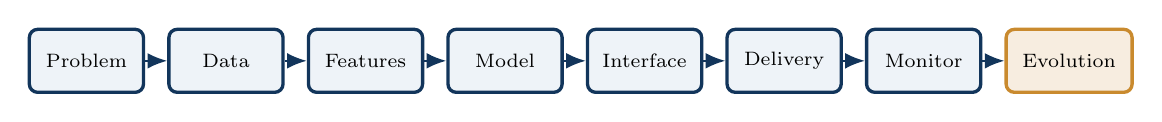
\begin{tikzpicture}[node distance=0.28cm]
  \node[flowbox, minimum width=1.45cm, minimum height=0.8cm] (problem) {\scriptsize Problem};
  \node[flowbox, minimum width=1.45cm, minimum height=0.8cm, right=of problem] (data) {\scriptsize Data};
  \node[flowbox, minimum width=1.45cm, minimum height=0.8cm, right=of data] (features) {\scriptsize Features};
  \node[flowbox, minimum width=1.45cm, minimum height=0.8cm, right=of features] (model) {\scriptsize Model};
  \node[flowbox, minimum width=1.45cm, minimum height=0.8cm, right=of model] (interface) {\scriptsize Interface};
  \node[flowbox, minimum width=1.45cm, minimum height=0.8cm, right=of interface] (delivery) {\scriptsize Delivery};
  \node[flowbox, minimum width=1.45cm, minimum height=0.8cm, right=of delivery] (monitor) {\scriptsize Monitor};
  \node[accentbox, minimum width=1.6cm, minimum height=0.8cm, right=of monitor] (evolution) {\scriptsize Evolution};
  \foreach \a/\b in {problem/data,data/features,features/model,model/interface,interface/delivery,delivery/monitor,monitor/evolution} {
    \draw[arrow] (\a) -- (\b);
  }
  \end{tikzpicture}

  \vspace{0.5em}
  \begin{block}{Today in the course}
  \textbf{Focus:} #1

  \textbf{Bridge:} #2
  \end{block}

  \begin{columns}[T]
  \column{0.48\textwidth}
  \begin{block}{Fraud case}
  {\footnotesize #3}
  \end{block}
  \column{0.48\textwidth}
  \begin{block}{Pasteurization case}
  {\footnotesize #4}
  \end{block}
  \end{columns}

  \vspace{0.3em}
  {\footnotesize \textbf{Course thread:} #5}
  \coursefooter
  \end{frame}
}

\newcommand{\classclosingframe}[4]{
  \begin{frame}{From This Class to the Next}
  \begin{block}{What stays with us}
  #1
  \end{block}

  \begin{columns}[T]
  \column{0.48\textwidth}
  \begin{block}{Project use}
  {\footnotesize #2}
  \end{block}
  \column{0.48\textwidth}
  \begin{block}{Next connection}
  {\footnotesize #3}
  \end{block}
  \end{columns}

  \vspace{0.3em}
  {\footnotesize \textbf{Course thread:} #4}
  \coursefooter
  \end{frame}
}

\tikzset{
  flowbox/.style={
    rounded corners=3pt,
    draw=courseblue,
    fill=courseice,
    very thick,
    minimum width=2.2cm,
    minimum height=0.9cm,
    align=center,
    font=\small
  },
  accentbox/.style={
    rounded corners=3pt,
    draw=coursegold,
    fill=coursegold!15,
    very thick,
    minimum width=2.2cm,
    minimum height=0.9cm,
    align=center,
    font=\small
  },
  arrow/.style={
    -{Latex[length=2.5mm,width=2mm]},
    thick,
    draw=courseblue
  }
}


\title{Class 17: Evaluation and Decision-Making}
\author{\coursename}
\date{}

\begin{document}

\frame{\titlepage \coursefooter}

\begin{frame}{Agenda}
\begin{itemize}
\item Evaluation must match the task, not the other way around.
\item Why accuracy can fail badly on rare-event problems.
\item From a prediction to a decision: what interfaces must communicate.
\item Thresholds, uncertainty, and operational cost.
\item Where trust in a model interface breaks down.
\end{itemize}
\coursefooter
\end{frame}

\begin{frame}{Learning goals}
\learninggoals{
\begin{itemize}
\item Choose evaluation metrics that reflect the real decision, not a generic leaderboard score.
\item Explain why accuracy is misleading under class imbalance.
\item Distinguish a prediction from a decision, and identify what a decision-support interface must expose.
\item Recognize the practical failure modes that erode trust in a served model.
\end{itemize}
}
\coursefooter
\end{frame}

\coursecontextframe
{Evaluating models against the real task, and turning scores into trustworthy decisions.}
{Class 16 gave us tracked, comparable model runs. This class asks whether the winning run is actually good for the decision it supports, and how that decision reaches a human or a downstream system.}
{In the fraud case, the key question is how to score rare events with metrics and thresholds that reflect the cost of a missed fraud versus a false alarm.}
{In the pasteurization case, a dashboard must communicate sensor state and model output together so an operator can act, not just observe a number.}
{The course thread now shifts from tracked experimentation to decision quality and operational trust.}

\begin{frame}{Evaluation must match the task}
\begin{itemize}
\item Imbalanced classification needs precision, recall, PR-AUC, and threshold analysis, not accuracy alone.
\item Regression needs error-magnitude metrics such as MAE or RMSE, chosen for the unit that matters operationally.
\item Calibrated probabilities matter whenever a downstream action depends on confidence, not just the predicted class.
\item Operational cost matters as much as any single numerical score.
\end{itemize}
\coursefooter
\end{frame}

\begin{frame}{Fraud dataset reality: extreme class imbalance}
\centering
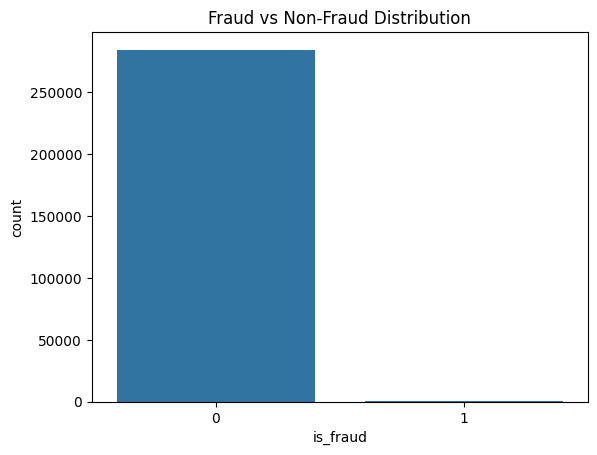
\includegraphics[height=0.72\textheight]{images/class05_fraud_class_balance.png}

{\scriptsize From `Credit_Card_Fraud_Detection_Solution.ipynb`: the first modeling challenge is not algorithm choice but the rarity of the positive class.}
\coursefooter
\end{frame}

\begin{frame}[fragile]{Repository example: fit, predict, and inspect errors}
\begin{lstlisting}[style=coursepython]
y_pred = best_model.predict(X_test_scaled)

print("Confusion Matrix:")
print(confusion_matrix(y_test, y_pred))

print("\nClassification Report:")
print(classification_report(y_test, y_pred))
\end{lstlisting}
\begin{itemize}
\item From `Credit_Card_Fraud_Detection_Solution.ipynb`: the confusion matrix exposes missed fraud cases directly, which a single accuracy number cannot.
\item The classification report opens the door to threshold and cost-sensitive evaluation.
\end{itemize}
\coursefooter
\end{frame}

\begin{frame}{Model interpretation: top feature importances}
\centering
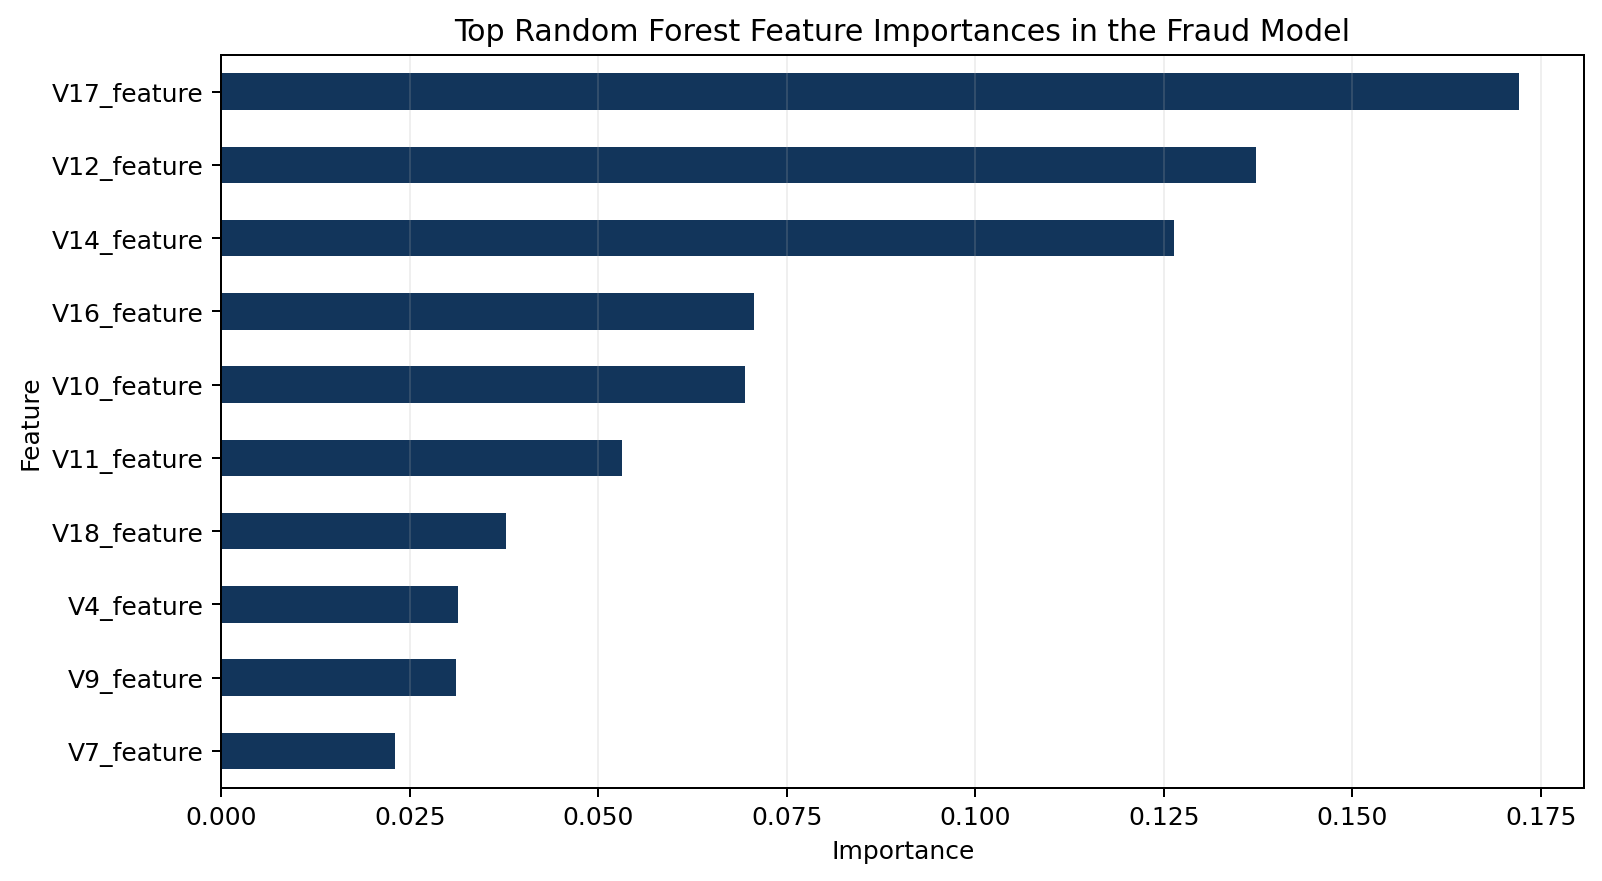
\includegraphics[height=0.7\textheight]{images/class05_feature_importance.png}

{\scriptsize Generated from the saved `streamlit/model.pkl`: tree-based models can highlight influential variables, but importance is still not the same as causality.}
\coursefooter
\end{frame}

\begin{frame}{Why accuracy can fail badly}
\begin{block}{Fraud example}
If only 0.2\% of transactions are fraudulent, a model that predicts ``legitimate'' every time may look highly accurate while being operationally useless.
\end{block}
\begin{itemize}
\item This is why threshold, recall, and precision are part of the engineering conversation, not an afterthought.
\end{itemize}
\coursefooter
\end{frame}

\begin{frame}{Distribution shape interacts with evaluation}
\centering
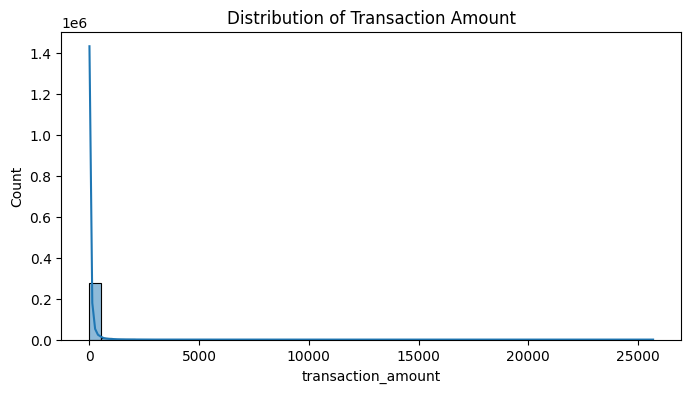
\includegraphics[height=0.72\textheight]{images/class05_transaction_amount_hist.png}

{\scriptsize The transaction amount distribution is highly skewed, a reminder that evaluation, scaling, and threshold choice all interact with each other.}
\coursefooter
\end{frame}

\begin{frame}{A model creates value only through an interface}
\begin{itemize}
\item A trained model that nobody can call or interpret has limited practical value, however good its offline metrics look.
\item An interface makes predictions available to users, services, and operational workflows.
\item The interface also shapes trust: input checks, response format, and clarity all matter as much as the metric that selected the model.
\end{itemize}
\coursefooter
\end{frame}

\begin{frame}{Prediction is not the final decision}
\begin{itemize}
\item A fraud score suggests escalation, not guilt.
\item A process alert suggests investigation, not automatic shutdown.
\item Interfaces should communicate uncertainty, threshold logic, and next actions whenever possible.
\end{itemize}
\begin{block}{Engineering implication}
The threshold that turns a probability into a decision is itself a design choice, not a byproduct of the model.
\end{block}
\coursefooter
\end{frame}

\begin{frame}[fragile]{Repository example: threshold-driven decision support}
\begin{lstlisting}[style=coursepython]
if st.button("Predict Fraud Risk"):
    prediction = model.predict(scaled)[0]
    probability = model.predict_proba(scaled)[0][1]

    if prediction == 1:
        st.error(f"Fraud Probability: {probability:.2%}")
    else:
        st.success(f"Fraud Probability: {probability:.2%}")
\end{lstlisting}
\begin{itemize}
\item From `streamlit/pages/App_Credit_Card.py`: the interface exposes both the decision and the probability behind it.
\item A human user needs labels, context, and actionable feedback, not raw class labels or JSON.
\end{itemize}
\coursefooter
\end{frame}

\begin{frame}{What a better dashboard should include}
\begin{itemize}
\item A visible explanation of what the model does and does not do.
\item Controls that reflect meaningful business inputs, not arbitrary technical internals.
\item Results that support action: alert, score, trend, or explanation.
\item Consistent links to data provenance, model version, or monitoring signals.
\end{itemize}
\coursefooter
\end{frame}

\begin{frame}{Where trust breaks down}
\begin{itemize}
\item The interface hides uncertainty behind a single confident-looking number.
\item The inputs shown to users do not match the assumptions the model was trained under.
\item The threshold was chosen once, informally, and never revisited as the data changed.
\item The dashboard makes a demo model look authoritative when it has not been validated for that purpose.
\end{itemize}
\coursefooter
\end{frame}

\begin{frame}{Repository connections}
\repoactivity{
\begin{itemize}
\item `Credit_Card_Fraud_Detection_Solution.ipynb` supplies the evaluation workflow this class is grounded in.
\item `streamlit/pages/App_Credit_Card.py` turns the same model into a threshold-driven, human-facing decision.
\item Both artifacts share one model and one scaler, so evaluation and decision-making must stay consistent with each other.
\end{itemize}
}
\coursefooter
\end{frame}

\begin{frame}{Discussion prompt}
\begin{block}{Question}
The fraud model has high recall but noticeably lower precision at the deployed threshold. Should we ship it as-is?
\end{block}
\begin{itemize}
\item This forces students to separate metric quality from decision quality and operational cost.
\item It also motivates the online adaptation and serving discussions in Classes 18 and 20.
\end{itemize}
\coursefooter
\end{frame}

\begin{frame}{Papers and materials}
\readinglist{
\href{https://scikit-learn.org/stable/modules/model_evaluation.html}{scikit-learn model evaluation guide};\
\href{https://dl.acm.org/doi/10.1145/2347736.2347755}{Domingos (2012), A Few Useful Things to Know About Machine Learning};\
\href{https://www.oreilly.com/library/view/designing-machine-learning/9781098107956/}{Chip Huyen, Designing Machine Learning Systems};\
\href{https://docs.streamlit.io/}{Streamlit documentation}.
}
\coursefooter
\end{frame}

\classclosingframe
{\begin{itemize}
\item Metrics are decision tools, chosen to reflect the real task, not decorative scoreboards.
\item A prediction becomes a decision only once thresholds, uncertainty, and interface design are made explicit.
\item Trust in a model interface is earned through validation, clarity, and honest communication of limits.
\end{itemize}}
{Project teams should now be able to defend both the metric they optimized and the threshold or interface behavior built on top of it.}
{Class 18 asks what happens when the data underneath a validated model starts to change: online learning and concept drift.}
{A model is only as trustworthy as its evaluation today and its ability to keep being evaluated as the world changes.}

\end{document}
